% vim: set tw=78 sts=2 sw=2 ts=8 aw et ai:
\documentclass{workshop}

% Comentează liniile de mai jos în cazul în care nu există cod de inclus.
\usepackage{code/highlight}
\usepackage{color}        % dacă e folosit highlight
\usepackage{alltt}        % dacă e folosit highlight

\title[Sesssion 7]{Session 7}
\subtitle{Introduction to Networking}
\author{Daniel Băluță, Irina Preșa}
\date{10 July 2012}

\begin{document}

% Arătăm numărul frame-ului
\setbeamertemplate{footline}[frame number]

\frame{\titlepage}

% NB: Secțiunile nu sunt marcate vizual, ci doar apar în cuprins
\section{Intro}
\begin{frame}{Network Stack}
\begin{figure}
  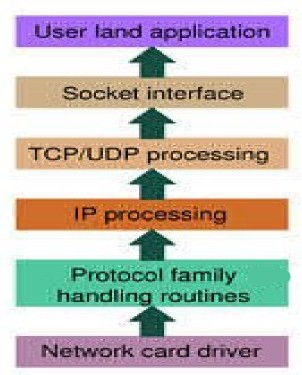
\includegraphics[scale=0.35]{img/stack.jpg}
\end{figure}
\end{frame}

\section{Package Structure - Skbuff}
\begin{frame}{Package Structure - Skbuff}
\input{code/skbuf}
\end{frame}

\begin{frame}{Package Structure - Skbuff}
\input{code/skbuff}
\begin{figure}
  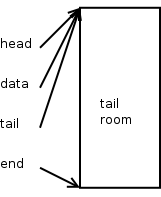
\includegraphics[scale=0.35]{img/1.png}
\end{figure}
\end{frame}

\begin{frame}{Package Structure - Skbuff}
\input{code/skbuff}
\begin{figure}
  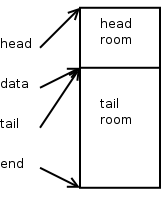
\includegraphics[scale=0.35]{img/2.png}
\end{figure}
\end{frame}

\begin{frame}{Package Structure - Skbuff}
\input{code/skbuff}
\begin{figure}
  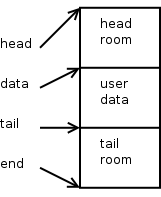
\includegraphics[scale=0.35]{img/3.png}
\end{figure}
\end{frame}

\begin{frame}{Package Structure - Skbuff}
\input{code/skbuff}
\begin{figure}
  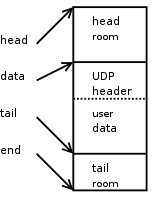
\includegraphics[scale=0.5]{img/4.png}
\end{figure}
\end{frame}

\begin{frame}{Package Structure - Skbuff}
\input{code/skbuff}
\begin{figure}
  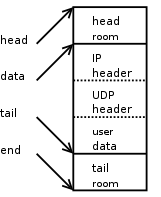
\includegraphics[scale=0.5]{img/5.png}
\end{figure}
\end{frame}

\section{Socket and Operations}
\begin{frame}{Socket and Operations}
\begin{figure}
  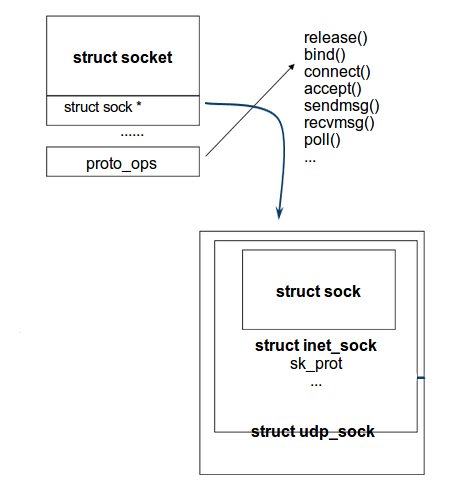
\includegraphics[scale=0.45]{img/socket.png}
\end{figure}
\end{frame}

\section{Register a New Protocol}
\begin{frame}{Register a New Protocol}
\begin{itemize}
\item Create Socket\\
\input{code/create}
\item First Receive Routine\\
\input{code/rcv}
\item Custom Sock Structure\\
\input{code/sock}
\end{itemize}
\end{frame}

\section{Send/Receive Flow}
\begin{frame}{Network Interrupts}
\begin{figure}
  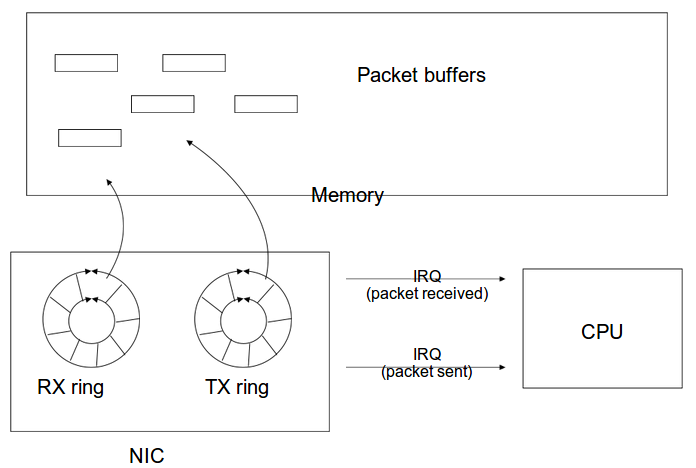
\includegraphics[scale=0.35]{img/rxtx.png}
\end{figure}
\end{frame}

\begin{frame}{Send}
\begin{itemize}
\item create transmission socket and connect.
\item create skbuff package structure.
\item put package in TX ring.
\end{itemize}
\end{frame}

\begin{frame}{Receive}
\begin{itemize}
\item bind a "listening" socket.
\item on receive call, wait until a package is available in the socket's
receive queue.
\item in receive interrupt handler add package to RX ring and schedule a softirq.
\item from the softirq handler, call the first receive routine (associated
    with the protocol) that moves a packet from RX to the destination socket's receive queue.
\end{itemize}
\end{frame}

\section{Keywords}
\begin{frame}{Keywords}
\begin{itemize}
\item kernel stack
\item skbuff
\item socket
\item RX/TX rings
\end{itemize}
\end{frame}

\section{Resources}
\begin{frame}{Resources}
\begin{itemize}
  \item \href{http://vger.kernel.org/~davem/skb.html}{How SKB's work}
  \item \href{http://www.haifux.org/lectures/217/netLec5.pdf}{Linux Kernel Networking}
  \item \href{http://www.scribd.com/doc/3471003/Linux-Networking-Internals}{Linux Networking Internals}
\end{itemize}
\end{frame}

\section{Questions}

\end{document}
